\documentclass[reprint,aps,prb,floatfix,longbibliography,amsmath,amssymb]{revtex4-2}
\usepackage{graphicx}
\usepackage{bm}
\usepackage{xcolor}
\usepackage[colorlinks=true,linkcolor=blue!60!black,citecolor=blue!60!black,urlcolor=blue!60!black,
  pdftitle={Designing the liquid region of Shakti artificial spin ice},pdfauthor={Changyeon Won}]{hyperref}

\newcommand{\dd}{\mathrm{d}}
\newcommand{\ii}{\mathrm{i}}
\newcommand{\ee}{\mathrm{e}}
\newcommand{\Kas}{\mathsf{K}}
\newcommand{\cK}{\mathcal{K}}
\newcommand{\hh}{\mathfrak{h}}
\newcommand{\qf}{q_{\rm f}}
\newcommand{\Pmax}{P_{\max}}
\newcommand{\lnt}{\ln(1+\sqrt2)}

\begin{document}

\title{Designing the liquid region of Shakti artificial spin ice}

\author{Changyeon Won}
\email{cywon@khu.ac.kr}
\affiliation{Department of Physics, Kyung Hee University, Seoul 02447, Republic of Korea}

\date{\today}

\begin{abstract}
The ground states of Shakti artificial spin ice are domino tilings, so a finite array splits into frozen regions and a liquid region whose shape is set by the boundary. We show that the cut and the edge termination of the array fix the boundary height of the tiling, and we use this dictionary to design the liquid region. Only axis cuts through the plaquette blocks and 45$^\circ$ cuts at even offset force order. Convex corner cuts then move and resize the arctic circle without changing its shape, whereas reflex corners reshape it: in plus-shaped samples with arm reach $n$ and half-width $c$ the liquid region is bounded by an algebraic curve that we give in closed form for $n/3<c<n/\sqrt2$. At finite temperature, edge plaquettes that close into vortices and unhappy boundary vertices act as boundary monomers, and their energy reduces to point sources at the sample corners. A square with two adjacent edges along block boundaries is therefore a temperature switch: it is completely frozen for $J/2T>m\ln(1+\sqrt2)$, where $J$ is the unhappy-vertex energy and $m$ the number of edge plaquettes that can close, and it becomes liquid throughout as the temperature rises. We solve the scaling limit of this switch by a hodograph transformation and confirm it with exact Pfaffian calculations, and we show that a square cut through the blocks realizes the boundary-vacancy model of the Aztec diamond. The results are rules for choosing the position, size, shape, and temperature window of the liquid region in nanomagnet arrays.
\end{abstract}

\maketitle

%==========================================================================
\section{Introduction}\label{sec:intro}
%==========================================================================

Artificial spin ices are lithographic arrays of single-domain nanomagnets whose moments act as Ising spins on the edges of a lattice~\cite{Wang2006,Nisoli2013RMP,Skjaervo2020}. In the Shakti geometry not all vertices can reach their lowest-energy state at once~\cite{Morrison2013,Chern2013}. Every rectangular plaquette contains exactly one unhappy three-leg vertex in a ground state, which it shares with a perpendicular neighbor, so the unhappy vertices form a dimer covering of the plaquette lattice. This mapping explains the extensive degeneracy, the emergent ice rule, and the classical topological order seen in Shakti arrays~\cite{Chern2013,Gilbert2014,Lao2018}.

Dimer coverings of the square lattice are domino tilings, and domino tilings of finite regions are known for their boundary-induced order. In the Aztec diamond the tiling is frozen into four brick phases outside an inscribed circle and is disordered, or liquid, inside it~\cite{EKLP1992,Jockusch1998,Cohn1996}. The mechanism is general. The boundary fixes the height function of the tiling, and the height inside follows from a variational principle~\cite{Cohn2001,KOS2006,Kenyon2007}. Frozen and liquid regions, and the arctic curve between them, have been computed for many domains, including the Aztec diamond with a cut corner~\cite{ColomoPronko2013,FerrariVeto2021}, the L-shaped domain~\cite{CPS2019,CharlierClaeys2025}, and a pentagon~\cite{ColomoPronko2024}, and the tangent method and harmonic parametrizations give arctic curves for general polygons~\cite{ColomoSportiello2016,Astala2020,KenyonPrause2020,Kuchumov2026}. In a companion paper we found that Shakti arrays with straight edges behave as Aztec diamonds below a crossover temperature that decreases with their size~\cite{KimVorticity}.

In a nanomagnet array the boundary is a design choice. Lithography fixes where the array is cut and which islands are kept at the edge, and the array is equilibrated at a temperature chosen by the experimenter. This raises a design question that the mathematical results do not answer by themselves: which liquid regions can be built from cuts and terminations of the Shakti lattice, and how do they respond to temperature? Two ingredients are missing. One is the dictionary from the island-level geometry of an edge to the boundary height of the tiling. The other is the finite-temperature behavior of open edges, where a plaquette can avoid its unhappy vertex.

Here we supply both and use them to design the liquid region. We show that the cut and the edge termination fix the boundary height, and that only axis cuts through the plaquette blocks and 45$^\circ$ cuts at even offset force order (Sec.~\ref{sec:model}). Convex corner cuts move and resize the arctic circle but keep it a circle, by a box rule that holds at every size (Sec.~\ref{sec:convex}). Reflex corners are needed to change its shape; for plus-shaped samples we derive the arctic curve in closed form and locate the two thresholds at which it appears and returns to a circle (Sec.~\ref{sec:reflex}). At finite temperature the edge energies reduce to point sources of the height at the corners. A square with two adjacent edges along block boundaries is then a temperature switch, frozen below a temperature set by the constant $\lnt$ and liquid throughout above it; we solve its scaling limit (Sec.~\ref{sec:switch}). The same reduction shows that a square cut through the blocks realizes the boundary-vacancy model of the Aztec diamond~\cite{WonVacancies} (Sec.~\ref{sec:vacancy}). Section~\ref{sec:discussion} collects the design rules and states where each result holds. Derivations and numerical methods are given in the Appendixes.

%==========================================================================
\section{Shakti ground states as domino tilings}\label{sec:model}
%==========================================================================

\subsection{Plaquettes, dimers, and heights}

We use the Shakti lattice as a basketweave of $1\times2$ rectangular plaquettes: $2\times2$ blocks of two parallel plaquettes, with the block orientation alternating like a checkerboard [Fig.~\ref{fig:cuts}(a)]. Islands sit on the unit edges, except on the middle edge of each plaquette. Vertices have coordination $z=2$, 3, or 4. We work with the vertex model of Ref.~\cite{KimVorticity}: an unhappy $z=3$ vertex costs $J$, and type-II and charged vertices cost $\Delta J$ with $\Delta=3$. Temperatures are in units with $k_B=1$.

In a ground state every plaquette contains one unhappy vertex, shared with a perpendicular plaquette~\cite{Morrison2013,Chern2013,Lao2018}. We call this pair a dimer. Mapping horizontal (H) plaquettes to black cells and vertical (V) plaquettes to white cells of a checkerboard turns the dimer covering into a domino tiling; the map is a $45^\circ$ rotation with a factor $\sqrt2$~\cite{KimVorticity}. The energy of a ground state is $J$ times the number of dimers.

The height function $h$ of the tiling~\cite{Thurston1990} lives on the vertices. In Shakti coordinates $(X,Y)$ its macroscopic slope $(\partial_Xh,\partial_Yh)$ lies in the slope square $[-1,1]^2$ (the Newton polygon). The four corners of the square are the four ice phases, the brick tilings in which all dominoes have the same orientation and offset [Fig.~\ref{fig:cuts}(b)]. The $90^\circ$ rotation about a block corner exchanges H and V plaquettes and maps $h\to-h$. It permutes the four corners of the slope square cyclically, and likewise its four edges.

\begin{figure*}[t]
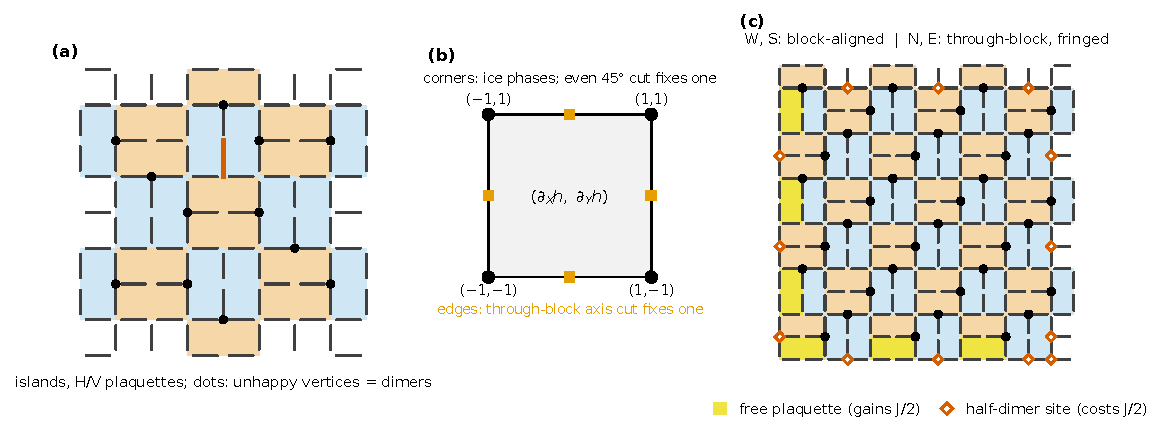
\includegraphics[width=\textwidth]{figures/fig1_cuts.pdf}
\caption{The cut and the termination of a Shakti array set the boundary of its domino tiling. (a)~Islands (bars) and plaquettes, H in orange and V in blue. In a ground state each plaquette shares one unhappy vertex (dot) with a perpendicular neighbor, which makes the pair a dimer. Red bar: the stem island of one plaquette. (b)~Slope square of the height function. Its corners are the four ice phases; a through-block axis cut fixes one component of the slope (an edge of the square, squares), and an even $45^\circ$ cut fixes the whole slope (a corner, dots). (c)~Ground state of a corner switch ($L=12$): the west and south edges are block-aligned, the north and east edges are cut through the blocks with fringed termination. Plaquettes without their stem island are free (yellow) and gain $J/2$. Half-dimer sites (diamonds) are boundary vertices that can become unhappy while covering a single plaquette, at a cost of $J/2$; they matter only at $T>0$.}
\label{fig:cuts}
\end{figure*}

\subsection{Boundary heights of straight cuts}

The boundary height of a cut sample follows from a counting rule. Walk along the boundary counterclockwise, with the sample on the left. Each unit edge of a plaquette whose perpendicular neighbor across that edge lies outside the sample is a dangling edge. Then
\begin{equation}\label{eq:D1}
  h(B)-h(A)=\sum_{e\in[A,B]}\sigma(p_e),
\end{equation}
where $p_e$ is the plaquette that owns the dangling edge $e$, and $\sigma=+1$ for H and $-1$ for V plaquettes. Physically, Eq.~\eqref{eq:D1} counts the candidate unhappy vertices that the cut has moved outside the sample, separately for H and V plaquettes. Because every dimer contains one H and one V plaquette, a tiling exists only if the sample has equal numbers of H and V plaquettes.

A straight cut is periodic, so its boundary slope depends only on its direction and on its offset modulo 4 relative to the lattice. Counting Eq.~\eqref{eq:D1} over one period gives Table~\ref{tab:cuts}. The slope along a cut of direction $(X,Y)$ can at most reach the support $|X|+|Y|$ of the slope square in that direction. Only two families reach it. Axis cuts at odd offset, which run through the middle of the blocks (through-block edges), reach a face of the slope square: they fix one component of the slope, as the staircase edges of an Aztec diamond do. The $45^\circ$ cuts at even offset reach a corner and fix the whole slope, so a single ice phase lines the edge. All other directions and offsets stay below the support, and the liquid region touches such an edge.

The reason is local. A cut is extremal only if all its dangling edges belong to plaquettes of one orientation. In a through-block cut whole half-blocks of one orientation line the edge, and in an even $45^\circ$ cut only plaquettes of one orientation protrude, like the teeth of a saw. The two directions are the mirror and glide lines of the p4g symmetry of the lattice; along any other direction H and V plaquettes alternate. Kasteleyn counts~\cite{Kasteleyn1961,Temperley1961} confirm the classification: through-block squares of side 8, 12, and 16 have $2^6$, $2^{15}$, and $2^{28}$ tilings, the numbers for Aztec diamonds of order 3, 5, and 7, and a $45^\circ$ square with four even edges has exactly one tiling.

\begin{table}[b]
\caption{\label{tab:cuts}Boundary slope of straight cuts, as the height rise per primitive lattice vector along the cut, for the four offsets $k$ modulo 4 (fringed termination). The support $|X|+|Y|$ is the largest possible value. Bold entries reach it.}
\begin{ruledtabular}
\begin{tabular}{cccccc}
Direction & $k=0$ & $k=1$ & $k=2$ & $k=3$ & Support \\
\hline
$(1,0)$ & 0 & \textbf{1} & 0 & \textbf{1} & 1 \\
$(1,1)$ & $\bm{-2}$ & 0 & \textbf{2} & 0 & 2 \\
$(2,1)$ & 1 & 0 & 1 & 0 & 3 \\
$(3,1)$ & 0 & 0 & 2 & 2 & 4 \\
$(3,2)$ & 0 & 1 & 0 & 1 & 5 \\
$(4,1)$ & 2 & 1 & 2 & 1 & 5 \\
\end{tabular}
\end{ruledtabular}
\end{table}

\subsection{Stem islands and free plaquettes}

Table~\ref{tab:cuts} assumes that every plaquette is paired. At an open edge this need not be so. Each plaquette has exactly one island that ends perpendicularly at the middle of its outer long side; we call it the stem island [Fig.~\ref{fig:cuts}(a), red]. In the bulk the stem island makes that point a $z=3$ vertex, which is the source of the frustration. If the cut removes the stem island, the point has $z=2$ and the plaquette can close its circulation without an unhappy vertex. We call such a plaquette freeable, and free when it is unpaired.

The ground states are then the dimer coverings in which every plaquette with a stem island is paired, and the ground-state energy is $J$ times the minimal number of dimers. Each free plaquette lowers the energy by $J/2$ relative to a paired one. Integer programming of the vertex model over all island spins agrees with this rule for all 44 samples we tested, including axis boxes of all four offsets, $45^\circ$ rhombi of 16 offsets, plus-shaped samples, octagons, tilted squares, and edges with randomly removed stem islands.

A free plaquette shifts the boundary height. Removing it from the tiled region changes the dangling edges on its perimeter, and Eq.~\eqref{eq:D1} gives
\begin{equation}\label{eq:D2}
  \delta h=-4\,\sigma(p)
\end{equation}
across the free plaquette $p$, independently of how many of its edges were exposed. The termination therefore decides the boundary. With fringed termination, which keeps the islands of the cut plaquettes, all stem islands survive and Table~\ref{tab:cuts} holds. With clean termination, which keeps only complete plaquettes, through-block edges acquire freeable plaquettes at density $1/4$, whose steps of 4 cancel the geometric slope; these edges become flat, $45^\circ$ edges likewise lose their extremal slope, and the sample is liquid up to the edge. Block-aligned edges, cut along block boundaries, have slope 0 by Table~\ref{tab:cuts}, but their freeable plaquettes are all free in the ground state [Fig.~\ref{fig:cuts}(c)]; by Eq.~\eqref{eq:D2} they raise the slope to the face value, so a block-aligned square is an Aztec diamond at $T=0$, as found in Ref.~\cite{KimVorticity}. In what follows through-block and $45^\circ$ edges are fringed.

%==========================================================================
\section{Convex cuts move the arctic circle}\label{sec:convex}
%==========================================================================

Because the slope lies in $[-1,1]^2$, every tiling obeys the Lipschitz bound $|h(q)-h(p)|\le\|q-p\|_1$, with $\|\cdot\|_1$ the $\ell_1$ distance in Shakti coordinates. This gives a rule that holds at every size.

\emph{Box rule.} If two boundary points $A$ and $B$ satisfy $h(B)-h(A)=\|B-A\|_1$, every point $q$ of the axis-parallel box with diagonal $AB$ has $h(q)=h(A)+\|q-A\|_1$. The box is frozen in one ice phase.

The proof is one line: for $q$ in the box $\|B-q\|_1+\|q-A\|_1=\|B-A\|_1$, so both Lipschitz inequalities must be equalities. On the lattice the same argument holds with the lattice distance, which makes the frozen region exact cell by cell. The same inequality is the tiling condition: if two boundary points violate it, the sample has no tiling.

Consider a square $|X|,|Y|\le a$ with through-block edges whose corners are cut by $45^\circ$ edges at even offsets $d_{\rm NE}$, $d_{\rm NW}$, $d_{\rm SW}$, and $d_{\rm SE}$ (the cut NE is $X+Y=d_{\rm NE}$, and so on). Along a $45^\circ$ edge the height changes by 2 per lattice vector, the largest possible value, so the far end of each cut and the points of one adjacent axis edge form extremal pairs. By the box rule each cut freezes a strip along one of its two neighboring axis edges. Which one depends on the offset class of the cut, $d\equiv2$ or $d\equiv0\pmod4$ (Appendix~\ref{app:box}). Applied to all cuts, the rule gives the octagon rule:
\begin{enumerate}
\item If two cuts freeze strips along the same axis edge, the sample has no tiling.
\item Otherwise each cut pushes its axis edge inward, and the sample is tileable only if the remaining rectangle is a square.
\item The remaining square is an Aztec diamond. The rest of the sample is frozen exactly.
\end{enumerate}
For four cuts of class $d\equiv2\pmod4$ the remaining square is
\begin{equation}\label{eq:octagon}
  X\in[a-d_{\rm SW},\,d_{\rm NE}-a],\qquad Y\in[a-d_{\rm SE},\,d_{\rm NW}-a],
\end{equation}
with the condition $d_{\rm NE}+d_{\rm SW}=d_{\rm NW}+d_{\rm SE}$; for class $d\equiv0$ the pinwheel winds the other way.

Convex corner cuts therefore move and resize the arctic circle without changing its shape (Fig.~\ref{fig:octagons}). The four offsets set the center and the radius independently: in Eq.~\eqref{eq:octagon} the center is at $[(d_{\rm NE}-d_{\rm SW})/2,(d_{\rm NW}-d_{\rm SE})/2]$ and the radius is $(d_{\rm NE}+d_{\rm SW})/2-a$. Cuts of mixed class are allowed when at most three corners are cut [Fig.~\ref{fig:octagons}(d)]; with four cuts of mixed class two of them always claim the same axis edge, and no tiling exists. Because the frozen strips are exact, the rule holds for arrays of any size, which makes it directly usable for small lithographic samples. We confirmed it for all 8500 valid octagons with $(a,b)=(13,13)$, $(17,13)$, $(13,9)$, and $(17,9)$ (rectangles $|X|\le a$, $|Y|\le b$): the 211 tileable ones have the predicted remaining square cell by cell, and the other 8289 have no tiling.

\begin{figure*}[t]
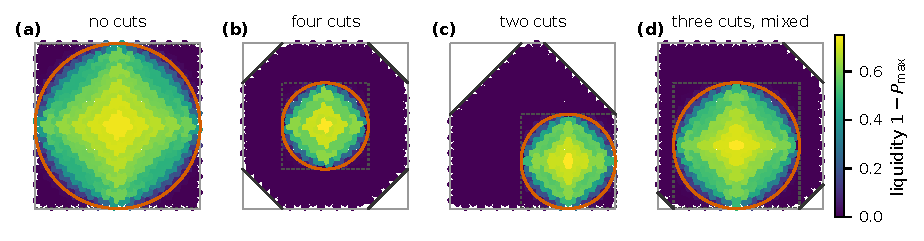
\includegraphics[width=\textwidth]{figures/fig2_octagons.pdf}
\caption{Convex corner cuts move and resize the arctic circle without changing its shape. Exact liquidity $1-\Pmax$ (Kasteleyn) of octagonal samples with through-block axis edges $|X|,|Y|\le21$ and even $45^\circ$ cuts at offsets $(d_{\rm NE},d_{\rm NW},d_{\rm SW},d_{\rm SE})$: (a)~no cuts, (b)~$(32,32,32,32)$, (c)~$(24,24,42,42)$, (d)~$(32,42,38,36)$, which mixes the two offset classes. Red: circle inscribed in the remaining square (dashed) predicted by the octagon rule. Here and in Figs.~\ref{fig:switch} and \ref{fig:vacancy}, $\Pmax$ is the largest pairing probability of a plaquette; all values are exact.}
\label{fig:octagons}
\end{figure*}

%==========================================================================
\section{Reflex corners reshape it}\label{sec:reflex}
%==========================================================================

A non-circular liquid region requires a reflex corner. We take the plus-shaped sample: the square $|X|,|Y|\le n$ with the four corner squares $|X|,|Y|>c$ removed, all edges through-block. Its arms have reach $n$ and half-width $c$.

\emph{Thresholds.} Along an arm the upper and lower edges have $\partial_Xh=+1$ and $-1$, so the height difference across the arm decreases linearly from $2c$ at the tip to $2(2c-n)$ at the root. The Lipschitz bound across the root requires $2(2c-n)\ge-2c$, so the plus is tileable if and only if
\begin{equation}\label{eq:third}
  c\ge n/3 .
\end{equation}
At $c=n/3$ the two reflex corners at the root of each arm form an extremal pair and the neck freezes. At the other end, the Aztec solution of the full square is frozen outside the circle $X^2+Y^2=n^2$. If the removed corner squares lie entirely outside it, that is, for $c\ge n/\sqrt2$, the restriction of the Aztec solution satisfies the boundary conditions of the plus, and we argue that it is the solution; the liquid region is then the full circle. For a single removed corner the tangency at this point is a third-order phase transition of the free energy~\cite{ColomoPronko2013}.

\emph{Arctic curve.} Between the thresholds the curve follows from the structure of the variational problem~\cite{Kenyon2007}. In the liquid region the complex slope is constant along straight lines, and the arctic curve is the envelope of a family of tangent lines
\begin{equation}\label{eq:tangent}
  X\cos\nu+Y\sin\nu=H(\nu),
\end{equation}
with normal angle $\nu$ and support $H$ (Appendix~\ref{app:tangent}). A boundary edge with normal $\nu_e$ is a tangent line with $H(\nu_e)$ equal to its distance from the origin. For the Aztec diamond $H=n$ and the envelope is the circle. Uniformizing the liquid region by a disk with boundary angle $\theta$, the normal angle is the phase of a Blaschke product of some degree $d$, and $H(\theta)$ is a trigonometric polynomial of degree $d$ divided by the squared modulus of the Blaschke denominator. The $90^\circ$ rotation, which maps $h\to-h$, restricts the degree of a fourfold-symmetric sample to $d=1,5,9,\dots$ (Appendix~\ref{app:tangent}).

The plus has 12 edges, but $d=5$ provides 20 axis-parallel tangents. The extra eight sit at the reflex corners. There the ice phases fixed by the two meeting edges are opposite corners of the slope square, so a third ice phase must lie between them, and its two boundaries are the continuations of the meeting edges. The arctic curve is tangent to these continuations, which we call hidden tangents. This reflex-corner condition is the one assumption beyond the variational principle. With it the symmetric family is
\begin{align}\label{eq:family}
  \nu&=5\theta+2\arctan\frac{p\sin4\theta}{1-p\cos4\theta},\nonumber\\
  H&=\frac{a_0+a_4\cos4\theta}{1+p^2-2p\cos4\theta},
\end{align}
and the conditions $H=n$ on the arm tip, $H=c$ on the arm side, and $H=-c$ on the hidden tangent fix $p$, $a_0$, and $a_4$. All three are rational functions of one parameter $\tau\in(0,\sqrt2)$,
\begin{equation}\label{eq:closed}
  \frac cn=\frac{\tau^2+2\tau+2}{6+4\tau-\tau^2},\qquad p=\frac{1-\tau-\tau^2}{1+\tau},
\end{equation}
with $a_0$ and $a_4$ given in Appendix~\ref{app:tangent}. Equation~\eqref{eq:closed} reproduces both thresholds: $\tau\to0$ gives $c/n=1/3$ and $p=1$, and $\tau=\sqrt2$ gives $c/n=1/\sqrt2$ and $p=-1$. The curve is algebraic of class 10, as the general theory of polygonal domains predicts it to be algebraic~\cite{Astala2020}; what is specific here is the explicit form and its realization in the Shakti lattice.

Figure~\ref{fig:plus} compares Eq.~\eqref{eq:closed} with exact pairing probabilities. Each reflex corner carries a frozen pocket in which three ice phases meet, bounded by two arcs of the curve [Fig.~\ref{fig:plus}(d)]. The pockets shrink as $c$ grows and disappear at $c=n/\sqrt2$, where the curve returns to the circle. For $n=241$ and $481$ the misclassified cells lie in a band along the curve whose width is 1--2\% of $n$, and the band narrows with size (Appendix~\ref{app:numerics}). The reflex-corner condition has an independent check. Applied to the L-shaped domain, which has one reflex corner, the same tangent family reproduces the arctic curve obtained by Colomo, Pronko, and Sportiello with the tangent method of the six-vertex model~\cite{CPS2019}, cusps included (Appendix~\ref{app:tangent}).

\begin{figure*}[t]
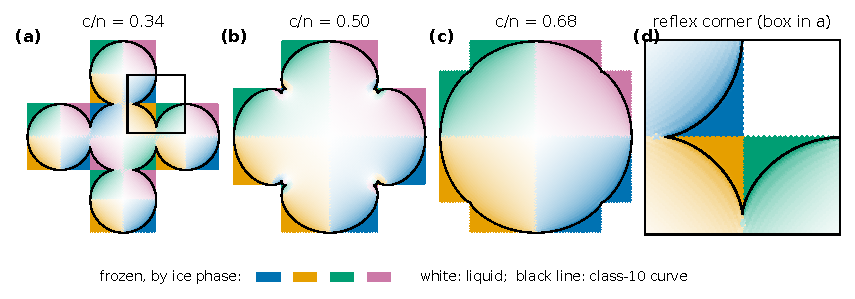
\includegraphics[width=\textwidth]{figures/fig3_plus.pdf}
\caption{Reflex corners make the liquid region non-circular. (a)--(c)~Plus-shaped samples with arm reach $n=241$ and half-width $c$, from exact pairing probabilities (urban-renewal recursion, $6.6\times10^4$ to $1.0\times10^5$ plaquettes). Frozen plaquettes are colored by their ice phase, the orientation of the dominant pairing; liquid plaquettes fade to white. Black: the curve of Eq.~\eqref{eq:closed}. (d)~Reflex corner of (a): a frozen pocket where three ice phases meet, bounded by two arcs of the curve. Below $c/n=1/3$ the plus has no tiling, and above $1/\sqrt2$ the curve is the full circle.}
\label{fig:plus}
\end{figure*}

%==========================================================================
\section{Switching with temperature}\label{sec:switch}
%==========================================================================

\subsection{Boundary model}\label{sec:bmodel}

At $T>0$ the open edges are the first to respond. A freeable plaquette that pairs costs $J/2$, and so does a second kind of boundary excitation. A boundary $z=3$ vertex whose unhappy state covers only one plaquette, because the other plaquette it would join lies outside the sample, makes that plaquette a half dimer [Fig.~\ref{fig:cuts}(c), diamonds]. We call such vertices half-dimer sites. They exist on all edges, block-aligned and through-block alike; the same sites set the crossover temperature of straight-edged arrays~\cite{KimVorticity}. A plaquette with a half-dimer site is unpaired by the tiling but carries an unhappy vertex, so relative to a paired plaquette it costs $J/2$.

The low-temperature physics is that of a boundary model: a dimer model in which plaquettes on the outer face can be monomers. A free plaquette has fugacity $\ee^{J/2T}$ and an occupied half-dimer site has fugacity $w\,\ee^{-J/2T}$, where the multiplicity $w=1$ or 2 counts the boundary vertices that can play this role for a given plaquette (Appendix~\ref{app:pfaffian}). Since all monomers lie on the outer face, the partition function is a Pfaffian~\cite{Giuliani2016},
\begin{equation}\label{eq:Z}
  Z=\mathrm{Pf}(\Kas+M),
\end{equation}
where $\Kas$ is the Kasteleyn matrix and $M$ couples the monomer sites (Appendix~\ref{app:pfaffian}). We evaluate Eq.~\eqref{eq:Z} in exact rational arithmetic, which is needed because frozen samples defeat double precision.

The temperature scale follows from counting. The number $m$ of freeable plaquettes grows linearly with the side $L$, and the entropy that their pairing releases grows as $L^2$, so the switch occurs at $T\sim J/L$. The scaling variable is
\begin{equation}\label{eq:q}
  q=\frac{J}{2mT},
\end{equation}
which we call the source strength, for reasons given in Sec.~\ref{sec:corner}. At this temperature a bulk excitation, which costs at least $J$, has weight $\ee^{-2qm}$ and is suppressed exponentially in the size. We tested the boundary model against the exact density of states of the vertex model for the corner switch introduced below, with $L$ up to 20 (Appendix~\ref{app:vertex}). The ground state is unique up to a global spin reversal in both. Every state of the first excited level of the vertex model, at energy $J$ above the ground state, is a boundary-model state, except for a single state at a corner. Without the half-dimer sites the boundary model would miss most of this level. From the second level on, the vertex model has additional states, and their relative weight decreases with $L$.

\subsection{Which rectangles switch}

We computed all 256 rectangles obtained by giving each of the four edges one of four offsets (Table~\ref{tab:rect}). Even offsets give block-aligned edges, which carry freeable plaquettes; odd offsets give through-block edges. Grouped by symmetry, only one class switches [Fig.~\ref{fig:switch}(a)]. If two adjacent edges are block-aligned and the other two are through-block, the ground state is unique, with every freeable plaquette free, and the sample is completely frozen at $T=0$ for all 64 offset combinations. At high temperature it is liquid. We call this sample the corner switch [Fig.~\ref{fig:cuts}(c)]. Two opposite block-aligned edges or three through-block edges admit no tiling, With three block-aligned edges the color imbalance usually fixes the number of free plaquettes, so these samples do not switch.

\begin{table}[t]
\caption{\label{tab:rect}Ground states of rectangles (sides 16--19) by edge type, block-aligned (B) or through-block (T), at $T=0$; BTBT has the two block-aligned edges opposite, BBTT adjacent. ``No tiling'' counts samples whose plaquettes cannot all be paired or freed; ``frozen'' counts samples with a unique ground state.}
\begin{ruledtabular}
\begin{tabular}{lcccc}
Edges & Samples & No tiling & Frozen & Liquid at $T=0$ \\
\hline
BBBB & 16 & 0 & 0 & circle \\
BBBT & 64 & 16 & 32 & none or most \\
BTBT & 32 & 32 & -- & -- \\
BBTT & 64 & 0 & 64 & none \\
BTTT & 64 & 64 & -- & -- \\
TTTT & 16 & 8 & 0 & circle \\
\end{tabular}
\end{ruledtabular}
\end{table}

\subsection{Edge energies are corner sources}\label{sec:corner}

The boundary energy of the corner switch is a function of two corner heights only. On each edge all monomers of one color carry the same energy. On the west edge the free plaquettes are white and the half-dimer sites black, on the south edge the reverse, and on the north and east edges only half-dimer sites exist, black and white respectively. By Eq.~\eqref{eq:D2} each monomer changes the boundary height by $\pm4$ according to its color, so the energy of an edge is proportional to the height difference between its two ends. Summing the four edges, the interior contributions cancel and
\begin{equation}\label{eq:Ebd}
  E_{\rm bd}=\frac J4\bigl[h({\rm NE})-h({\rm SW})\bigr]+\text{const}.
\end{equation}
The temperature thus enters the variational problem for the height only through a source at the corner SW and a sink at the corner NE, of strength proportional to $q$. Everywhere else the edges obey the natural boundary condition of zero normal current, as long as the monomer density stays in its allowed range; on the west and south edges both colors are allowed, on the north and east edges only one. This is the structure found for vacancies in the Aztec diamond, where four alternating corner sources appear~\cite{WonVacancies} [Fig.~\ref{fig:vacancy}(a)]. The reduction requires only that the monomer energy be uniform along each edge; different values on different edges change the source strengths but not the structure.

\begin{figure*}[t]
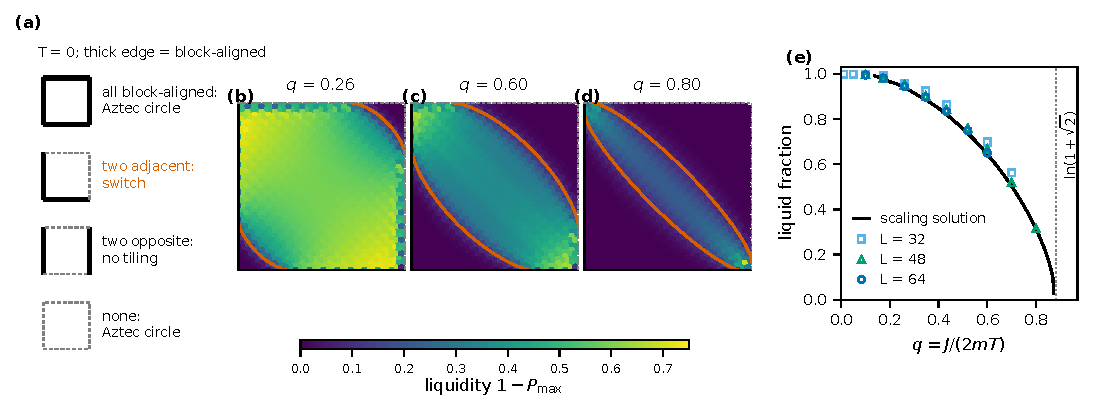
\includegraphics[width=\textwidth]{figures/fig4_switch.pdf}
\caption{A square with two adjacent block-aligned edges is a temperature switch. (a)~Ground states of rectangles by edge type (thick: block-aligned): only two adjacent block-aligned edges give a unique ground state that melts. (b)--(d)~Exact liquidity of the corner switch ($L=48$, boundary model) at three source strengths $q=J/2mT$, with the frozen boundaries of the scaling solution (red). (e)~Liquid fraction versus $q$ for $L=32$, 48, and 64 (points) and the scaling solution (line). The sample freezes completely at $q=\ln(1+\sqrt2)$ (dotted).}
\label{fig:switch}
\end{figure*}

\subsection{Scaling solution}

We solve the scaling limit of the corner switch by the hodograph method of Ref.~\cite{WonVacancies}, with new boundary data. Scale the sample to the unit square $0\le u,v\le1$ with SW at the origin. The diagonal $u=v$ is a mirror line, so it suffices to solve the triangle below it, bounded by the south edge, the east edge, and the diagonal. For domino tilings the slope is parametrized by a complex number $\omega$, and the Euler-Lagrange equation of the variational principle states that~\cite{Kenyon2007}
\begin{equation}\label{eq:burgers}
  v-\lambda(\omega)\,u=\Psi(\omega),\qquad \lambda(\omega)=\frac{2\omega}{1-\omega^2},
\end{equation}
with an analytic function $\Psi$. In the variable $\zeta=(\omega-\ii)/(\omega+\ii)$, where $\lambda=\ii(1-\zeta^2)/(1+\zeta^2)$, the liquid part of the triangle is mapped onto a fixed domain: the quarter disk $|\zeta|<1$, $-\pi/2<\arg\zeta<0$, with the segment $r_D<|\zeta|<1$ of the ray $\arg\zeta=-\pi/4$ removed. The real axis is the south edge between the frozen cap at SW and the corner SE, where the tangential slope is $(4/\pi)\arctan|\zeta|$; the imaginary axis is the east edge; $\zeta=0$ is the flat corner SE; the arc $0<\varphi<\pi/4$ of $\zeta=\ee^{-\ii\varphi}$ is the boundary of the SW cap and the arc $\pi/4<\varphi<\pi/2$ that of the NE cap; and the two sides of the removed segment are the two halves of the diagonal, which meet at the center. Temperature enters only through $r_D$.

With $Q=(\zeta^2+\zeta^{-2})/2$, $b=(r_D^{-2}-r_D^2)/2$, $P=(Q^2+b^2)^{1/2}$, and $P_1=(1+b^2)^{1/2}$, we write $v-\lambda(u-1)=-\hh/(\zeta+\zeta^{-1})$. The boundary conditions become $\mathrm{Re}\,\hh=0$ on both axes, $\mathrm{Im}\,\hh=0$ on the arcs, and $\mathrm{Im}\,\hh=-[(P_1^2-P^2)^{1/2}-1]^{1/2}$ on the diagonal. Removing the factor $(P^2-P_1^2)^{1/2}$ turns this mixed problem into a Cauchy integral,
\begin{align}\label{eq:sol}
  \hh&=\ii\sqrt{P^2-P_1^2}\;\cK(P),\nonumber\\
  \cK(P)&=\frac1\pi\int_{-b}^{b}\frac{\kappa(P')\,\dd P'}{P'-P},
\end{align}
with $\kappa(P')=[(P_1^2-P'^2)^{1/2}-1]^{1/2}/(P_1^2-P'^2)^{1/2}$. Finiteness of $(u,v)$ excludes any added homogeneous solution, and the symmetry that exchanges SW and NE together with $h\to-h$ makes $\cK$ odd, so no constant can be added either (Appendix~\ref{app:hodograph}). The frozen boundaries are the envelopes of the lines
\begin{equation}\label{eq:envelope}
  (u-1)\sin\varphi+v\cos\varphi=\tfrac12\sqrt{P_1^2-P^2}\;\cK(P),
\end{equation}
with $Q=\cos2\varphi$, and the SW cap meets the south edge at $X_1=1+\cK(P_1)$. The source strength follows from the flux of the height current from the corner SW, which an integration by parts reduces to
\begin{equation}\label{eq:qint}
  q=\lnt+\frac12\int_0^1\cK\bigl(\sqrt{Q^2+b^2}\bigr)\frac{\dd Q}{\sqrt{1-Q^2}} .
\end{equation}

Equation~\eqref{eq:qint} contains the freezing temperature. Since $\cK<0$, the integral lowers $q$ below $\lnt$, and it vanishes as $b\to0$, where the two caps fill the two triangles of the square. The sample is therefore completely frozen for
\begin{equation}\label{eq:freeze}
  \frac{J}{2T}>m\lnt .
\end{equation}
The constant comes from a single point: where the SW cap meets the diagonal, the complex slope is $\omega=\cot(\pi/8)=1+\sqrt2$. The exact counts confirm it independently: the number of states at the first excited level of the frozen sample grows as $\ee^{\kappa L}$ with $\kappa\to\lnt$, which gives the same freezing condition (Appendix~\ref{app:vertex}). At high temperature the caps shrink as $X_1\simeq1.27\,q$, close to the size $(4/\pi)q$ of an isolated frozen corner in Ref.~\cite{WonVacancies}, and the liquid fraction approaches 1 as $1-O(q^2)$.

Figure~\ref{fig:switch} compares the solution with exact calculations of the boundary model. The frozen boundaries of Eq.~\eqref{eq:envelope} follow the exact liquidity maps [Figs.~\ref{fig:switch}(b)--\ref{fig:switch}(d)], and the exact liquid fractions approach the scaling solution as $L$ grows [Fig.~\ref{fig:switch}(e) and Table~\ref{tab:switch}]. As the temperature rises, the liquid region opens along the diagonal from SE to NW and spreads until it fills the sample. The switch is complete in both directions: the sample is frozen in a single state below $T_{\rm f}=J/[2m\lnt]$ and liquid nearly everywhere at $q\ll1$. The only function in the solution that is not elementary is $\cK$; all other quantities are one-dimensional integrals over it. If the north and east edges are fixed instead, so that only the west and south edges carry monomers, the same method gives a solution in elementary functions; we record it in Appendix~\ref{app:hodograph} because Ref.~\cite{WonVacancies} refers to it.

\begin{table}[t]
\caption{\label{tab:switch}Liquid fraction of the corner switch: scaling solution and exact boundary model for three sizes.}
\begin{ruledtabular}
\begin{tabular}{cccccc}
$q$ & Scaling & $L=32$ & $L=48$ & $L=64$ \\
\hline
0.26 & 0.940 & 0.956 & 0.951 & 0.945 \\
0.433 & 0.820 & 0.862 & 0.841 & 0.834 \\
0.60 & 0.645 & 0.699 & 0.668 & 0.650 \\
0.70 & 0.50 & 0.562 & 0.519 & 0.500 \\
0.80 & 0.312 & -- & 0.315 & -- \\
\end{tabular}
\end{ruledtabular}
\end{table}

%==========================================================================
\section{Through-block squares and boundary vacancies}\label{sec:vacancy}
%==========================================================================

A square with four through-block edges, $1\le X,Y\le L+1$, has no freeable plaquettes. At $T=0$ it is the Aztec diamond of order $N=L/2-1$, with $2^{N(N+1)/2}$ ground states. It is not temperature independent, however: half-dimer sites sit on every second boundary cell of all four edges, $2N$ in total, each with multiplicity $w=2$ and with the color of the boundary cells of its edge. Since replacing a dimer by two monomers costs $J$, each monomer has fugacity $2\ee^{-J/2T}$. The edge colors alternate around the square, so Eq.~\eqref{eq:D2} gives four corner sources of alternating sign [Fig.~\ref{fig:vacancy}(a)]. The vertex model agrees exactly at the first excited level: the boundary model counts 768, 1\,966\,080, and 67\,645\,734\,912 states for $N=3$, 5, and 7, the same numbers as the vertex model.

This is the boundary-vacancy model of the Aztec diamond~\cite{WonVacancies}, in which every boundary cell can be vacant with fugacity $z$ and the scaling limit depends only on $x=2\log_2(1/z)/N$. Matching the fugacities,
\begin{equation}\label{eq:xmap}
  2\ee^{-J/2T}=2^{-xN/2},\qquad\text{that is,}\qquad \frac JT=(xN+2)\ln2 .
\end{equation}
The arctic circle starts to melt at $x=1$, which corresponds to $T_{\rm on}=J/[(N+2)\ln2]$. This is the crossover temperature that Ref.~\cite{KimVorticity} gives for arrays cut through the blocks; for block-aligned arrays, whose edges carry both free plaquettes and half-dimer sites, $N+4$ replaces $N+2$ [Eq.~(15) of Ref.~\cite{KimVorticity}]. Only half of the boundary cells carry sites here. We argue that this does not change the scaling limit: in the vacancy model the vacancy density never exceeds $1/2$, and the boundary term depends only on the net number of monomers on each edge, which is a height difference.

The exact calculation supports this (Fig.~\ref{fig:vacancy} and Table~\ref{tab:vacancy}). The uncompensated fraction $\sigma_N=1-\langle n_{\rm mono}\rangle/2N$ of the Shakti square, computed for $N$ up to 47, approaches the scaling function $\sigma_\infty(x)$ of Ref.~\cite{WonVacancies} from above, whereas the vacancy model approaches it from below. Extrapolations in $1/N$ agree with $\sigma_\infty$ to within 0.003--0.008, the spread between extrapolation forms. Below $T_{\rm on}$ the square shows the arctic circle; above it the frozen corners shrink and, as in the vacancy model, their size is set by the temperature rather than by the sample [Figs.~\ref{fig:vacancy}(b) and \ref{fig:vacancy}(c)]. A through-block square with fringed termination is thus a physical realization of the boundary-vacancy model, with $x=(J/T-2\ln2)/(N\ln2)$.

\begin{figure*}[t]
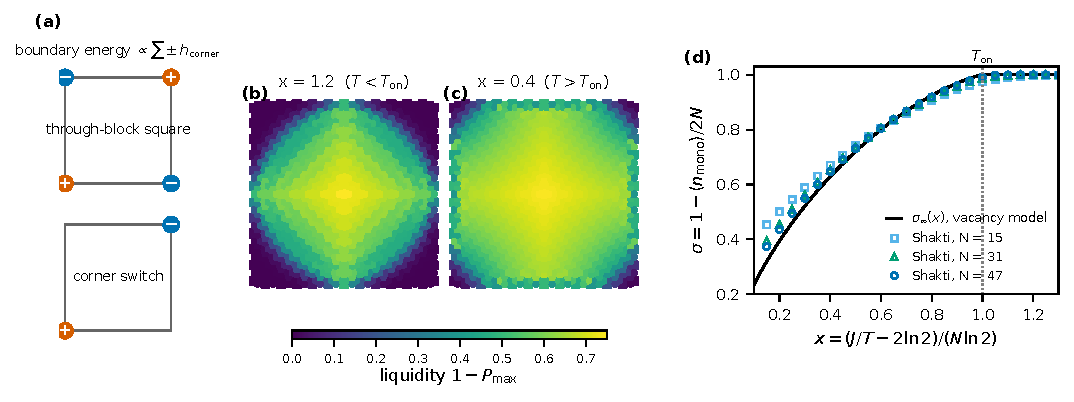
\includegraphics[width=\textwidth]{figures/fig5_vacancy.pdf}
\caption{Edge energies reduce to corner sources, and a through-block square realizes the boundary-vacancy model. (a)~Signs of the corner sources: alternating on the through-block square, one diagonal pair on the corner switch. (b), (c)~Exact liquidity of the through-block square ($N=23$, boundary model) below and above $T_{\rm on}$. (d)~Uncompensated fraction $\sigma=1-\langle n_{\rm mono}\rangle/2N$ for $N=15$, 31, and 47 (points) against the scaling function of the boundary-vacancy model~\cite{WonVacancies} (line), with $x=(J/T-2\ln2)/(N\ln2)$; $x=1$ is $T_{\rm on}$.}
\label{fig:vacancy}
\end{figure*}

\begin{table}[t]
\caption{\label{tab:vacancy}Uncompensated fraction $\sigma_N$ of the through-block square, its extrapolation (fit in $1/N$ and $1/N^2$, $N\ge23$), and the scaling function $\sigma_\infty$ of the boundary-vacancy model~\cite{WonVacancies}.}
\begin{ruledtabular}
\begin{tabular}{cccccccc}
$x$ & $N=7$ & 15 & 23 & 31 & 47 & Extrap. & $\sigma_\infty$ \\
\hline
0.3 & 0.640 & 0.589 & 0.571 & 0.561 & 0.549 & 0.523 & 0.521 \\
0.5 & 0.752 & 0.743 & 0.738 & 0.735 & 0.731 & 0.721 & 0.721 \\
0.7 & 0.847 & 0.860 & 0.865 & 0.866 & 0.867 & 0.868 & 0.868 \\
\end{tabular}
\end{ruledtabular}
\end{table}

%==========================================================================
\section{Discussion}\label{sec:discussion}
%==========================================================================

\emph{Design rules.} Table~\ref{tab:rules} collects what each geometric choice does to the liquid region. The position and size of the arctic circle are set by convex $45^\circ$ cuts, exactly and at every size. Its shape is set by reflex corners, with a window $n/3<c<n/\sqrt2$ for the plus in which frozen pockets of three ice phases appear. Whether it exists at all can be set by temperature, through block-aligned edges: a corner switch is frozen below $T_{\rm f}$ and liquid above it, and since $T_{\rm f}\propto1/m$ the size of the switch selects its temperature. Rules of this kind compose. For example, squares joined along a diagonal keep the balance of H and V plaquettes, whereas a straight neck between two squares breaks it, so composite samples are best built from diagonally overlapping squares.

\begin{table}[t]
\caption{\label{tab:rules}Design rules for the liquid region.}
\begin{ruledtabular}
\begin{tabular}{p{0.36\columnwidth}p{0.56\columnwidth}}
Choice & Effect \\
\hline
Termination & fringed: extremal edge; clean: flat edge, liquid touches it \\
Through-block axis edge & one slope component fixed; liquid touches at one point \\
Even $45^\circ$ edge & one ice phase along the edge \\
Convex $45^\circ$ cuts & move and resize the arctic circle, Eq.~\eqref{eq:octagon} \\
Reflex corners & non-circular curve; plus: $n/3<c<n/\sqrt2$, Eq.~\eqref{eq:closed} \\
Two adjacent block-aligned edges & frozen for $J/2T>m\ln(1+\sqrt2)$, liquid at high $T$ \\
Four through-block edges & arctic circle melts above $T=J/[(N+2)\ln2]$ \\
\end{tabular}
\end{ruledtabular}
\end{table}

\emph{Validity.} The results rest on different grounds, and we state them separately. The boundary-height dictionary, the box rule, and the octagon rule are exact statements about tilings; the stem-island rule, which connects them to the vertex model, was checked for 44 samples. The thresholds $c=n/3$ (proved) and $c=n/\sqrt2$ (argued) do not depend on the form of the curve. The curve of Eq.~\eqref{eq:closed} assumes the Kenyon-Okounkov structure of the variational problem and the reflex-corner condition; the latter is not proved, but it reproduces an independent result for the L-shaped domain, and the curve agrees with exact maps up to $n=481$. At finite temperature the boundary model is exact for the first excited level of the vertex model. From the second level on, the vertex model has additional states whose relative weight decreases with size; that they vanish in the scaling limit is supported by the exponential suppression of bulk excitations at $T\sim J/L$ but is not proved. The scaling solution assumes the structure of the hodograph domain; its predictions match the exact boundary model as $L$ grows, and the freezing constant is confirmed by the exact level counts. The correspondence with the boundary-vacancy model is numerical, supported by the argument that only net monomer numbers enter the boundary term. Finally, the vertex model neglects the long-range part of the dipolar interaction. Its main effect at an edge is to shift the monomer energies away from $J/2$. As long as the shift is uniform along each edge, the corner-source structure of Eq.~\eqref{eq:Ebd} survives with modified strengths.

\emph{Experiments.} Frozen regions are static vertex patterns, and the liquid region is where the pattern fluctuates. In thermally active Shakti arrays~\cite{Gilbert2014,Lao2018} the liquid region can therefore be imaged from the variance of repeated images or from an ensemble of annealed samples. The frozen pockets of the plus are a direct test of the reflex-corner condition, since three ice phases meet in a region of fixed relative size. The temperature switch requires equilibration at $T\sim J/L$, the same constraint as for $T_{\rm on}$ in Ref.~\cite{KimVorticity}; arrays of moderate size, a few tens of plaquettes across, are therefore best suited. Because $T_{\rm f}$ depends on $m$ alone, switches of different sizes on one chip would melt in sequence on heating.

%==========================================================================
\section{Conclusion}\label{sec:conclusion}
%==========================================================================

The cut and the termination of a Shakti array fix the boundary height of its domino tiling, so the liquid region can be designed. Convex cuts move and resize the arctic circle, reflex corners reshape it into an algebraic curve that we gave in closed form for the plus, and two adjacent block-aligned edges switch it on and off with temperature. The switching works because the energies of all edges reduce to point sources at the corners, so that the temperature enters only through one source strength; the scaling solution then gives the frozen and liquid regions at every temperature and the freezing condition $J/2T=m\lnt$. The same reduction makes the through-block square a realization of the boundary-vacancy model of the Aztec diamond. Open problems are a proof of the reflex-corner condition, a closed form of the function $\cK$, the suppression of bulk defects in the scaling limit, and the extension of the switch to samples with more than two block-aligned edges or with holes.

\begin{acknowledgments}
This research was supported by the National Research Foundation (NRF) of Korea funded by the Korean Government (NRF-2023R1A2C1006050). The author used Claude (Anthropic) to assist with writing code for the numerical computations and figures and with editing the manuscript; all results were checked by the author, who takes full responsibility for the content.
\end{acknowledgments}

\section*{Data availability}
The codes and data that support the findings of this article are openly available~\cite{repo}. Each figure is reproduced by one script listed in the repository.

\appendix

%==========================================================================
\section{Box rule and octagon rule}\label{app:box}
%==========================================================================

Let $A$ be the far end of a $45^\circ$ cut and $P$ a point of an adjacent axis edge. Along the cut the height changes by 2 per lattice vector and along the axis edge by 1 per unit length, the maximal values, so $h(P)-h(A)=\|P-A\|_1$ when the boundary path from $A$ to $P$ runs along the cut and then the axis edge with consistent signs. The box rule then freezes the box spanned by $A$ and $P$ for every $P$ on that edge up to the next cut, which is a strip along the edge. The signs are consistent for exactly one of the two axis edges adjacent to the cut. Counting edges counterclockwise, a cut of class $d\equiv2\pmod4$ freezes a strip along the edge before it (NE: east, NW: north, SW: west, SE: south), and a cut of class $d\equiv0$ along the edge after it (NE: north, NW: west, SW: south, SE: east). The cut NE then moves the east edge to $X=d_{\rm NE}-a$ (class 2) or the north edge to $Y=d_{\rm NE}-a$ (class 0), and similarly for the other corners. If one axis edge receives two strips, the far ends of the two cuts violate the Lipschitz bound and the sample has no tiling. For four cuts, avoiding this requires all cuts to choose the edge before them or all the edge after them, so four cuts of mixed class admit no tiling. The remaining rectangle must be a square, because around a rectangle with four face-extremal edges the boundary height closes only if the sides are equal.

%==========================================================================
\section{Tangent family and the plus}\label{app:tangent}
%==========================================================================

\emph{Characteristic lines.} In the liquid region the complex slopes $(z,w)$ lie on the spectral curve $P(z,w)=0$ and satisfy the complex Burgers equation $z_x/z+w_y/w=0$~\cite{Kenyon2007}. With $w=w(z)$ this reads $z_x+(zw'/w)z_y=0$, so $z$ is constant on straight lines, and the general solution is $x\,zP_z+y\,wP_w=Q(z)$ with an analytic function $Q$. For uniform dominoes, $P=1+z+w-zw$, and $z=\tan(\phi/2)$ turns these lines into Eq.~\eqref{eq:tangent} with $\nu=\phi-\pi/2$. The four values $z\in\{0,1,\infty,-1\}$ are the axis-parallel tangents, one for each face of the slope square.

\emph{Polygonal samples.} Mapping the liquid region onto the unit disk ($u=\ee^{\ii\theta}$ on the boundary), $z$ becomes a Blaschke product $B(u)$ of degree $d$, and $H(\theta)$ is a real trigonometric polynomial of degree at most $d$ divided by the squared modulus of the denominator of $B$. There are $4d$ axis-parallel tangents, and since $B$ is monotonic on the boundary the four face labels appear in cyclic order.

\emph{Degree restriction.} The $90^\circ$ rotation $R$ about a block corner maps $h\to-h$ and the slope $s\to-Rs$, a cyclic shift of the faces. For an $R$-symmetric sample, $R$ acts as $u\to\ii u$ on the disk, and in the variable $(z-\ii)/(z+\ii)$ the Blaschke product obeys $B(\ii u)=\ii B(u)$. Its zeros are invariant under multiplication by $\ii$, so $B(u)/u$ is a function of $u^4$ and $d=1+4k$. With mirror symmetry the parameters are real, $B(u)=u(u^4-p)/(1-pu^4)$ and $H\propto a_0+a_4\cos4\theta$, which is Eq.~\eqref{eq:family}.

\emph{Reflex corners.} At a convex corner the face label advances by one step, at a reflex corner by three, so each reflex corner carries two tangents that are not edges. Past the contact point of the upper side of an arm (slope component $\partial_Xh=+1$ fixed) the edge is lined by the ice phase $(+1,-1)$, and the side of the neighboring arm by $(-1,+1)$. These are opposite corners of the slope square and cannot touch along a line, so the phase $(-1,-1)$ lies between them. Two adjacent ice phases meet along a straight line normal to their slope difference: $X=c+\delta$ and $Y=c+\delta$ with the same $\delta$. For $\delta>0$ the phase $(-1,-1)$ would touch the edge, against the boundary condition; for $\delta<0$ the opposite phases would meet along a kinked line, which we exclude as non-minimizing. Hence $\delta=0$, and the arctic curve, which is tangent to the ice-ice boundaries where it meets them, is tangent to the continuations $X=c$ and $Y=c$ of the neighboring arm sides. The exclusion of $\delta<0$ and the tangency are the steps that are not proved.

\emph{Closed form.} The points where $B=-1$ satisfy a palindromic equation, which gives $2\cos\theta_2=[(1+p)+\sqrt{(1-p)^2+4}]/2$, and the rotation maps $B=\ii$ onto $B=1$, which gives $2\sin\theta_1=[\sqrt{(1-p)^2+4}-(1+p)]/2$. With $\tau=2\sin\theta_1$ and $\kappa_2=2\cos\theta_2$ one has $\tau\kappa_2=1-p$ and $\kappa_2-\tau=1+p$, hence $\kappa_2=(2+\tau)/(1+\tau)$, and the three conditions give Eq.~\eqref{eq:closed} and
\begin{align}
  \frac{a_4}{n}&=\frac{2(\tau^4+3\tau^3+3\tau^2+2\tau+2)}{(1+\tau)(6+4\tau-\tau^2)},\\
  \frac{a_0}{n}&=-\frac{\tau^6+2\tau^5-10\tau^4-28\tau^3-14\tau^2+8\tau+4}{(1+\tau)^2(6+4\tau-\tau^2)}.
\end{align}
The inverse is $\tau=[2\rho-1+\sqrt{10\rho^2-1}]/(1+\rho)$ with $\rho=c/n$. Points of the curve are $(X,Y)=H(\cos\nu,\sin\nu)+(H'/\nu')(-\sin\nu,\cos\nu)$, with primes denoting $\dd/\dd\theta$. The closed form agrees with a direct numerical solution of the three conditions to six digits.

\emph{L-shaped domain.} For the square $|X|,|Y|\le n$ with the quadrant $X>a$, $Y>b$ removed there are six edges and two hidden tangents, so $d=2$, $B(u)=\ee^{\ii\gamma}u(u-\beta)/(1-\bar\beta u)$, and $H$ is a degree-2 trigonometric polynomial over $|1-\bar\beta u|^2$. The seven real unknowns are fixed by the eight tangency conditions, one of which is implied by the closure of the boundary height; the system has solutions with residual $10^{-9}$. For $a=b=0.4n$ and $0.6n$ the resulting curve coincides with Eqs.~(4.15)--(4.17) of Ref.~\cite{CPS2019}, mapped by $(x,y)=((1+X/n)/2,(1-Y/n)/2)$, over its whole length including the two cusps; the largest difference, below $10^{-3}n$, is set by the resolution of the comparison. The cusps lie on the hidden tangents.

%==========================================================================
\section{Boundary Pfaffian}\label{app:pfaffian}
%==========================================================================

Number the monomer sites $1,\dots,s$ in the order in which a walk along the outer face meets them, and let $\ell_i$ be the fugacity of site $i$ relative to a paired plaquette: $\ell_i=\ee^{J/2T}$ for a freeable plaquette, $\ell_i=w_i\ee^{-J/2T}$ for a plaquette with half-dimer sites, and the sum of both if a plaquette has both. Then~\cite{Giuliani2016}
\begin{equation}
  Z=\mathrm{Pf}(\Kas+M),\qquad M_{ij}=-M_{ji}=G_iG_j\ell_i\ell_j\quad(i<j),
\end{equation}
where $G_i$ is the product of the Kasteleyn signs along the boundary path from site 1 to site $i$, so that $G_iG_j$ is the sign of a virtual edge $(i,j)$ drawn outside the sample. For an odd number of plaquettes we add one auxiliary site that is always a monomer. The multiplicity $w$ follows from the island geometry: a boundary $z=3$ vertex that touches a single plaquette contributes 2 if it has coordination 3 in the infinite lattice and 1 if it is a corner point of coordination 4, and a vertex that touches two plaquettes that are not neighbors contributes 1 to each of them that is not freeable. These weights were fixed by matching the endpoint statistics of the first excited level of the vertex model at $L=8$ and confirmed at $L=12$.

Frozen samples make the matrix nearly singular in double precision (samples of 300 plaquettes with a unique ground state gave non-integer numbers of free plaquettes), so we evaluate the Pfaffian in exact rational arithmetic with FLINT~\cite{flint}. At an integer fugacity $y=2^k$ the integer square root of $\det(\Kas+M)$ written in base $2^k$ has the state counts $c_j$, with $j$ monomers, as its digits, which gives the polynomial $Z(y)$ exactly. Probabilities follow from the inverse matrix. The formula agrees with brute-force sums over all monomer sets to $10^{-10}$ for block-aligned and through-block squares, a $45^\circ$ rhombus, and a plus, and for site-dependent weights at $L=4$ and 8.

%==========================================================================
\section{Vertex-model check}\label{app:vertex}
%==========================================================================

We computed the exact density of states $g(E)$ of the vertex model of the corner switch for $L=4$--20 with a vertex-by-vertex transfer matrix over all island spins (693 islands at $L=20$). The ground-state degeneracy is 2, the global spin reversal, for all sizes.

Enumerating all states of the first excited level ($1978$ states at $L=8$, $57\,230$ at $L=12$) shows that each has exactly two boundary vertices that are unhappy in it but not in the ground state, the two ends of a string. If both ends sit at freeable plaquettes, the state is a re-paired pair of free plaquettes, and the numbers of such states agree with the boundary model without half-dimer sites (64 and 1826). All other ends are half-dimer sites. With them the boundary model gives $g(E_{\rm gs}+J)/g(E_{\rm gs})=988$, 28\,614, and 859\,864 for $L=8$, 12, and 16, against 989, 28\,615, and 859\,865 for the vertex model; the one missing state is a string with a single end at a corner. At the second level the ratio of the vertex model to the boundary model is 1.264, 1.188, and 1.172 for the same sizes.

The number of states at the first level of the boundary model without half-dimer sites, which already sets the growth rate, behaves as $\ee^{\kappa L}L^{-\alpha}$ with local fits $\kappa=0.8791$, 0.8801, 0.8805, 0.8808 and $\alpha=0.433$--0.466 for $L$ up to 32, consistent with $\kappa=\lnt=0.8814$ and $\alpha=1/2$. One excitation costs $J$ and gains $T\kappa L$ in entropy, so the sample is frozen for $J/2T>m\lnt$ with $m=L/2$, as in Eq.~\eqref{eq:freeze}. The first level of the vertex model is larger by a nearly constant factor (15.5--15.8 for $L=8$--16), so its growth rate is the same.

Figure~\ref{fig:vertex} compares the mean excitation energy. The boundary model with half-dimer sites follows the vertex model, and the difference decreases with $L$ at all temperatures, from 0.186 at $L=8$ to 0.026 at $L=20$ for $q=0.433$. Without half-dimer sites the excitation energy is too small by a factor between 2 and 15.

\begin{figure}[t]
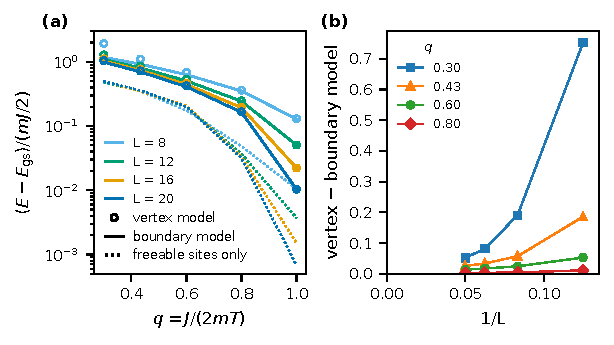
\includegraphics[width=\columnwidth]{figures/fig6_vertex.pdf}
\caption{The boundary model with half-dimer sites reproduces the vertex model (exact density of states, corner switch). (a)~Mean excitation energy per freeable plaquette for $L=8$--20: vertex model (circles), boundary model (lines), and boundary model with freeable plaquettes only (dotted). (b)~Difference between the vertex model and the boundary model versus $1/L$.}
\label{fig:vertex}
\end{figure}

%==========================================================================
\section{Hodograph solution}\label{app:hodograph}
%==========================================================================

\emph{Domain.} The method follows Appendix~B of Ref.~\cite{WonVacancies}. In the triangle below the diagonal, the south edge carries monomers between the end $X_1$ of the SW cap and the corner SE; there $\zeta=r$ is real and the natural boundary condition fixes the tangential slope $(4/\pi)\arctan r$. The east edge carries monomers of one color, and on it $\zeta$ is imaginary. The caps are bounded by the arcs of the unit circle, and the diagonal, a mirror line, is traced twice by the removed segment. That the liquid region maps onto this domain for all temperatures is an assumption, supported by the agreement with the exact maps. The map $Q=(\zeta^2+\zeta^{-2})/2$ followed by $P=(Q^2+b^2)^{1/2}$ opens the domain to a half-plane in which the axes, the arcs, and the diagonal are the intervals $|P|>P_1$, $b<|P|<P_1$, and $|P|<b$.

\emph{Uniqueness.} The difference of two solutions has the form $\ii(P^2-P_1^2)^{1/2}R(P)$ with $R$ real on the real axis. Finiteness of $(u,v)$ at every boundary point where $\zeta+\zeta^{-1}$ is finite and nonzero excludes poles of $R$ at finite $P$, and the behavior at $\zeta=0$, where $\zeta+\zeta^{-1}\simeq(2P)^{1/2}$, excludes growth. The reflection across the antidiagonal combined with $h\to-h$ requires $\cK(-P)=-\cK(P)$, which fixes the remaining constant to zero. Substituting $P'=P_1\sin\theta$ gives $\cK(P)=\pi^{-1}\int_{-\theta_b}^{\theta_b}(P_1\cos\theta-1)^{1/2}\dd\theta/(P_1\sin\theta-P)$ with $\cos\theta_b=1/P_1$, an elliptic integral. No point solution $\Psi=c_1+c_2\lambda$ satisfies the conditions on the south edge, the east edge, and the diagonal at once, which is why $\cK$ does not reduce to elementary functions. For small $b$, $\kappa$ becomes a semicircle density and $\cK\simeq[(P^2-b^2)^{1/2}-P]/\sqrt2$.

\emph{Temperature.} The flux form $\Omega=\frac12\int(\ln\omega\,\dd v-\ln\eta\,\dd u)$, with $1+\omega+\eta-\omega\eta=0$, is closed, and $\dd\eta/\eta=\lambda\,\dd\omega/\omega$. Integrating by parts, $\Omega=\frac12(v\ln\omega-u\ln\eta)-\frac12\int\Psi\,\dd\omega/\omega$. We integrate from the corner SE ($\zeta=0$, $\omega=\ii$) along the south edge and the SW cap to the point where the cap meets the diagonal ($\zeta=\ee^{-\ii\pi/4}$, $\omega=\eta=1+\sqrt2$). The boundary terms have zero real part at both ends. The term $-\ii\mu$ of $\Psi$ integrates to $\ln\eta$ and gives $\lnt$; the remainder is real only on the cap and gives the integral in Eq.~\eqref{eq:qint}. The result agrees with direct integration of the flux to four digits for $b\le2$ and is stable up to $b=200$. Table~\ref{tab:caps} lists values.

\begin{table}[t]
\caption{\label{tab:caps}Scaling solution of the corner switch: source strength and end of the SW cap on the south edge.}
\begin{ruledtabular}
\begin{tabular}{ccccccc}
$b$ & 0.05 & 0.3 & 1 & 2.315 & 10 & 200 \\
\hline
$q$ & 0.8792 & 0.8343 & 0.6417 & 0.4320 & 0.1958 & 0.0424 \\
$X_1$ & 0.9991 & 0.9701 & 0.7881 & 0.5449 & 0.2492 & 0.0540 \\
\end{tabular}
\end{ruledtabular}
\end{table}

\emph{Fixed-edge variant.} If the north and east edges carry no monomers, they are fixed at the ice phase of the NE corner, and only the west and south edges respond. The domain has the same shape, but the imaginary axis is now the empty part of the south edge, where the height is constant, and $\zeta=0$ is the point of the south edge where the slope vanishes. With $a\equiv1/P_1$ the solution is elementary,
\begin{equation}
  \Psi=v-\lambda u=-\ii\,\frac{\sqrt{2(P-P_1)/P_1}}{\zeta+\zeta^{-1}},
\end{equation}
obtained by adding to the trivial solution, in which everything collapses to the corner, the one homogeneous solution allowed by finiteness. On the south edge the frozen part ends at $u=a$, the monomer density decreases from 1 to 0 between $u=a$ and $u=\sqrt a$, and the edge is empty beyond. The two frozen boundaries are the branches $\mathcal{S}=\sin\chi$ and $\cos\chi$ of $\mathcal{S}\sqrt{1-\mathcal{S}^2}=a\sin\varphi\cos\varphi$, with $\mathcal{S}$ the support function measured from SW in the normal direction $(\sin\varphi,\cos\varphi)$ and $\sin2\chi=a\sin2\varphi$. The source strength is
\begin{equation}
  q=\int_0^\infty\frac{g(Q)-1}{Q^2-1}\,\dd Q,
\end{equation}
with $g(Q)=\{[1+(1-a^2+a^2Q^2)^{1/2}]/2\}^{1/2}$, which at $a=1$ equals $\lnt$, so this variant freezes at the same point. At high temperature the liquid region is a quarter of the arctic circle of the reflected sample, and the fraction of free plaquettes is $f(a)=(2\sqrt2a/\pi)\int_0^{\pi/2}\dd\theta\,[\sin^2\theta+(\sin^4\theta+4a^2\cos^2\theta)^{1/2}]^{-1/2}$. Integrating the temperature from the frozen side gives the entropy $0.086643$ at $a\to0$, equal to $(\ln2)/8$, the value for a quarter of the Aztec diamond of side $2L$; this value was not used in the solution. Exact calculations of this variant approach the predicted free fraction as $L$ grows; for $L=48$--96 the difference is between 0.001 and 0.01.

%==========================================================================
\section{Numerical methods}\label{app:numerics}
%==========================================================================

Pairing probabilities of samples up to a few thousand plaquettes were obtained from the inverse Kasteleyn matrix. Its accuracy, measured by the deviation of the summed pairing probabilities of a plaquette from 1, is $5\times10^{-14}$ for the plus with $n=31$ but $5\times10^{-6}$ at $n=61$ and of order 1 at $n=91$, because the condition number grows exponentially with the frozen area. For larger samples we used the generalized domino-shuffling (urban-renewal) recursion~\cite{Propp2003}, which involves only additions and multiplications of positive numbers and is carried out in logarithms. A plus is embedded in an Aztec diamond by covering the cells outside it with a fixed matching and giving weight zero ($\ee^{-600}$) to all other edges at those cells. The recursion agrees with Kasteleyn values to $10^{-15}$ for random weights, and the summed probabilities deviate from 1 by less than $10^{-14}$ at all sizes; $n=481$ (about $3.5\times10^5$ plaquettes) takes 85~s.

A plaquette is counted as frozen if $1-\Pmax<0.1$. Compared with the inside of the curve of Eq.~\eqref{eq:closed}, the misclassified plaquettes are 1.9\%, 1.4\%, 1.3\%, and 1.5\% for $n=241$ and $c=83$, 121, 145, and 165, and 1.0\% for $n=481$, $c=241$; none lies farther than 3--6 cells from the curve. Outside the curve the liquidity decays as $\exp[-\frac43(d/w)^{3/2}]$ with distance $d$; the fitted width $w$ grows as $n^{0.36}$ for $n=61$--481, close to the Airy exponent $1/3$. Liquidity maps of the corner switch and the through-block square were computed from the boundary Pfaffian in double precision, keeping only temperatures at which the summed probabilities deviate from 1 by less than $10^{-3}$; thermodynamic quantities were computed in exact arithmetic.

\bibliography{refs}

\end{document}
